%-----------------------------------------------------------------------------------------------
\section{Evaluation}
\subsection{Design}
\begin{frame}
\frametitle{Research Design - Data Structure} 
\begin{itemize}
	\item \textbf{3 cities - Reggio, Parma and Padova}
	\begin{itemize}
		\item Similar geographic location
		\item Parma more similar to Reggio in terms of culture and history
	\end{itemize}
	\bigskip
	\item \textbf{5 cohorts - Ages 6, 17, 30, 40 \&  50}
	\begin{itemize}
		\item Age 6: Children entering elementary school
		\item Age 17: Adolescents reaching maturity
		\item Age 31-32: Adults at first life milestone
		\item Age 40-41: Adults at second milestone. First to get access to ITC
		\item Age 53-58: Adults born before the Reggio Approach was implemented
	\end{itemize}
\end{itemize}
\end{frame} 

%-----------------------------------------------------------------------------------------------
\begin{frame}
\frametitle{Reggio Emilia, Parma, Padova} 
\begin{center}
\begin{figure}
\includegraphics[height=1.0\textheight]{include/3-cities-map.png}
%\caption{{Location of the city of Parma, Reggio Emilia, and Padova, Italy.}}
\end{figure}
\end{center}
\end{frame}
%-----------------------------------------------------------------------------------------------
\begin{frame}
\frametitle{Population-level Data}
\begin{itemize} 
\item \textbf{Demographic Data:} population, births, deaths, migration, age distribution, marital status,  household size and family composition

\item \textbf{Educational Data:}  educational attainment, infant, preschool and high school enrollment 

\item \textbf{Economic Data:} home ownership by type, labor force participation, employment by industry, employment by occupation , income distribution and poverty rates

\item \textbf{Election Statistics:} votes for Communist/Christian democracy parties

\item \textbf{Religion:}  religious vs civil marriages 

\end{itemize}
\end{frame}
%%-----------------------------------------------------------------------------------------------
\begin{frame}
\frametitle{Main Sources}
\begin{itemize}
\item \textbf{Tracking data available online:} from websites of local municipalities, provincial and regional offices, Italian Census Data (Istat), historical archive of elections etc.


\item \textbf{Collecting hard copy data:}
Municipality Statistical Offices (demographic and education data), Provincial Offices (educational data),
and Regional Istat Office (labor data, Census) 

\end{itemize}
\end{frame}
%%-----------------------------------------------------------------------------------------------
\begin{frame}
\begin{block}{Demographic Data: family composition}
This variable is available from Census 1991, 2001 and 2011. We will check earlier years in Istat Regional office we plan to visit next week. 
\end{block}

\begin{block}{Educational Data: infant, preschool and high school enrollment}
\begin{itemize}
\item We need to digitize data we have collected on preschool and high school enrollment
\item We will go to the municipality of Padova next week to collect more data on education
\item We have established contact with municipality of Parma and will visit there soon.
\end{itemize}
\end{block}
\end{frame}
%%-----------------------------------------------------------------------------------------------
\begin{frame}
\begin{block}{Economic Data: employment by occupation, income distribution, poverty rates}
\begin{itemize}
\item We will get this information on employment by occupation from Census Data per decade between 1971-2011.
\item We have established contact with Istat Regional Office and plan to visit there next week to get income distribution and poverty rates. From what we understand labor statistics are mostly collected from surveys which are representative only at provincial level (rather than in city levels) 
 
\end{itemize}
\end{block}
\end{frame}
%%-----------------------------------------------------------------------------------------------
\begin{frame} 
\frametitle{Sample by City and Cohort}
\begin{figure}[H]
\begin{center}
	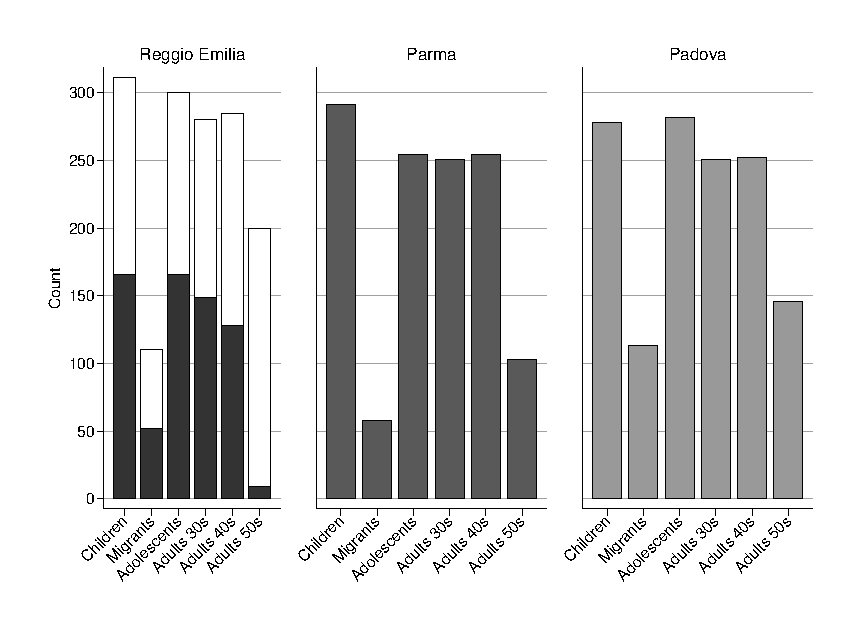
\includegraphics[width=.8\textwidth]{./include/sample}
\end{center}
\footnotetext{\scriptsize \noindent \textit{Note}: Number of individuals by cohort and city. In Reggio Emilia we differentiate between those who attended municipal preschool (black bars) and those who did not (white bars).}
\end{figure}
\end{frame}
%%-----------------------------------------------------------------------------------------------
\begin{frame}
\frametitle{Attendance Infant-toddler Centers (0-3)} 
\begin{center}
\begin{figure}
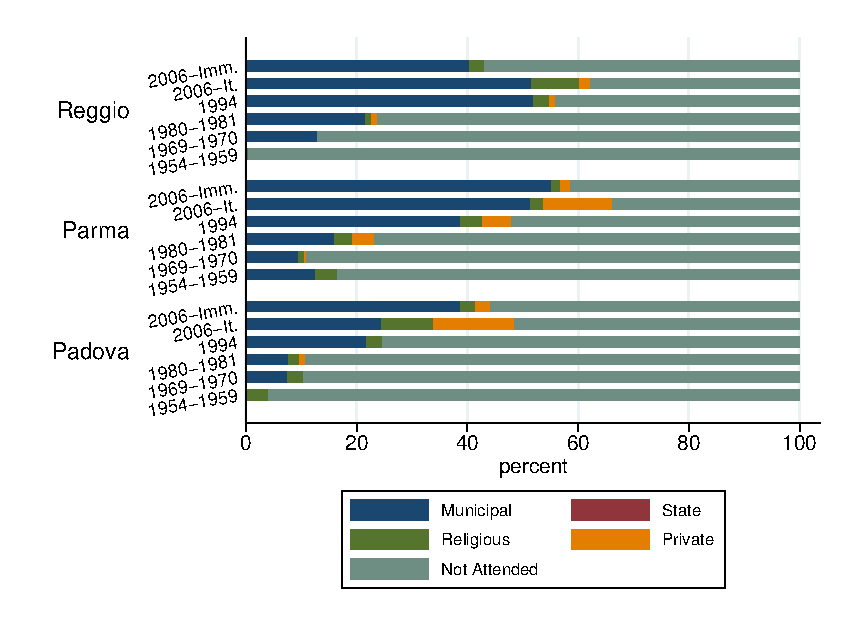
\includegraphics[width=1.15\textheight]{asiloType-Attend.eps}
%\caption{{Location of the city of Parma, Reggio Emilia, and Padova, Italy.}}
\end{figure}
\end{center}
\end{frame}
%------------------------------------------------------------------------------------------------
\begin{frame}
\frametitle{Attendance Preschools (3-6)} 
\begin{center}
\begin{figure}
\includegraphics[width=1.15\textheight]{maternaType-Attend.eps}
%\caption{{Location of the city of Parma, Reggio Emilia, and Padova, Italy.}}
\end{figure}
\end{center}
\end{frame}
%-------------------------------------------------------------------------------------------------
\begin{frame}
\frametitle{Research Design -Treatment} 
\underline{\textbf{Definition of Treatment}}
\begin{itemize}
	\item \textbf{Treated:} Those who attended Municipal schools in Reggio
	\smallskip
	\item \textbf{Control:} Those who didn't attend Municipal schools in Reggio
	\begin{itemize}
		\item Attended non-Municipal schools in Reggio
		\item Attended any school in Parma or Padova
		\item Attended no preschool in any city
	\end{itemize}
\end{itemize}
\bigskip
\underline{\textbf{Potential Issues:}}
\begin{itemize}
	\item Diffusion of Reggio Approach into control group
	\item Differential rates of diffusion over time, between schools, and across cities
\end{itemize}
\begin{block}{}
$\mathbf{\hookrightarrow}$ Recently conducted interviews to understand these differences
\end{block}

\end{frame}
%-----------------------------------------------------------------------------------------------